\documentclass[oneside]{ausarbeitung}
\bibliography{latexlit}


% ----------------------------------------------------------------------

\begin{document}

%--- Sprachauswahl
% Erlaubte Werte:
%   \selectlanguage{english}
%   \selectlanguage{ngerman}
\selectlanguage{ngerman}

%--- Art der Arbeit
% Erlaubte Werte:
%   \Praxissemesterbericht
%   \Projektbericht
%   \Bachelorarbeit
%   \Seminararbeit
%   \Masterarbeit

\Projektbericht

%--- Studiengang:
% Erlaubte Werte:
%   \Informatik
%   \Elektronik
%   \DataScience
\Informatik

\title{Scavenger Hunt}

\author{Hikmet Gözaydin; Niklas Fichtner}
\matrikelnr{85987; 85822}

%--- Ist der Erstbetreuer (\examinerA) an der Hochschule ein Professor?
% Erlaubte Werte:
%   \examinerIsAProfessortrue   % Ja
%   \examinerIsAProfessorfalse  % Nein
\examinerIsAProfessortrue   % Nein

%--- Betreuer
\examinerA{Dr. Marc Hermann}
%\examinerB{Prof.~Dr.~Ulrich~Klauck}

%--- Einreichungsdatum
\date{14. August 2025}

%--- Angaben zur Firma
% Auskommentieren, wenn die Arbeit nicht bei einer ext. Firma gemacht wurde.
% \companyname{Beispielfirma}
% \industrialsector{Beispielbranche}
% \department{Beispielabteilung}
% \companystreet{Beispielstr. 1}
% \companycity{12345 Musterstadt}

%--- Angaben zum Betreuer bei dieser Firma
% \advisorname{Name des Betreuers}
% \advisorphone{(01234) 567-890}
% \advisoremail{name@company.xxx}

%--- Titelseite Anzeigen
\maketitle
\cleardoublepage

%---
\pagenumbering{roman}
\setcounter{page}{1}

%--- Firmendaten Anzeigen
% Auskommentieren, wenn die Arbeit nicht bei einer ext. Firma gemacht wurde.
% \makeworkplace
% \cleardoublepage

%--- Eidesstattliche Erklärung anzeigen
\makeaffirmation
\cleardoublepage

%--- Sperrvermerk (Funktioniert nur bei externen Bachelor- oder Masterarbeiten.)
\makeconfidentialclause
\cleardoublepage

%---
\begin{abstract}

Im Rahmen dieses Projekts wurde eine webbasierte Anwendung entwickelt, die es Nutzern ermöglicht, spielerisch Orte und Angebote einer Hochschule zu entdecken.  
Das Projekt basiert auf einem schlanken, modernen Technologie-Stack mit React im Frontend, FastAPI im Backend und PostgreSQL als Datenbank.  

Ein zentrales Ziel war es, das System serverseitig zuverlässig und reproduzierbar mittels Docker-Containern bereitzustellen.  
Dadurch konnte ein stabiler, wartbarer und plattformunabhängiger Betrieb sichergestellt werden, der einfache Updates und Erweiterungen ermöglicht.  

Die Nutzeroberfläche wurde benutzerfreundlich gestaltet und unterstützt verschiedene Medientypen (Text, Video, Bild, Audio, GPS), um abwechslungsreiche Aufgaben und Hinweise bereitzustellen.  
Darüber hinaus wurden umfangreiche Funktionen zur Verwaltung von Hunts, Nutzer-Accounts und GPS-basierten Interaktionen implementiert.  

Abschließend wurde die Anwendung durch User-Tests validiert, die wertvolle Rückmeldungen lieferten und zur Optimierung beitrugen.  
Das Projekt liefert damit eine praxisnahe Lösung für die Kombination von spielerischem Lernen, Orientierung auf dem Campus und moderner Softwareentwicklung.

\end{abstract}
%-----------------------------------------------------------------------
\cleardoublepage
\tableofcontents

%---
\listoffigures

%---
\listoftables

%---
% \lstlistoflistings

%---
% \listofabbreviations
\begin{acronym}[Bsp.]  % Längstes Kürzel in der nachfolgenden
                       % Liste um die Breite der Spalte für die
                       % Abkürzungen zu bestimmen.

%% Eintrag: \acro{Referenzname}[Kürzel]{Langform}
%% Im Text wird die Abkürzung dann mit \ac{Referenzname} benutzt.
\acro{rup}[RUP]{Rational Unified Process}
%\acro{bsp}[Bsp.]{Beispiel}
\end{acronym}
%---


\cleardoublepage
\pagenumbering{arabic}
\setcounter{page}{1}

% ----------------------------------------------------------------------
\chapter{Einleitung}
\label{cha:einleitung}


\section{Motivation}
\label{sec:motivation}

Die Projektarbeit gibt uns die Möglichkeit, gelernte Theorie praktisch anzuwenden: Anforderungen analysieren, Lösungen entwerfen, implementieren, testen und deployen. In der Gruppe haben wir unterschiedliche Fähigkeiten kombiniert, gemeinsam Entscheidungen getroffen und typische Arbeitsabläufe wie Versionskontrolle, Code-Reviews und iterative Verbesserungen geübt.

Unser Projekt verfolgt das Ziel, Orte und Angebote der Hochschule spielerisch kennenzulernen. Teilnehmende erhalten eine Abfolge von Aufgaben in Form von Text, Video, Bild, Audio oder GPS. Jede gelöste Station führt zur nächsten, optional helfen Hinweise. 

So verbindet das Projekt Lernen, Orientierung auf dem Campus und praktische Softwareentwicklung in einem realistischen Szenario.

\section{Problemstellung und -abgrenzung}
\label{sec:problemstellung}

Ausgangspunkt war ein bereits vorhandenes Projekt, das wir übernommen haben. Die Codebasis war allerdings ziemlich unübersichtlich, und das Starten der Umgebung hing an einer GUI, was reproduzierbare Builds erschwerte und auf macOS teilweise gar nicht funktionierte. Die alte Architektur war für unseren Use-Case überdimensioniert und an einigen Stellen unsauber. Für unser Projekt haben wir uns deshalb für einen schlankeren Stack entschieden: React im Frontend, FastAPI im Backend, PostgreSQL als Datenbank. Damit ist die Lösung wesentlich wartbarer, leichter zu deployen und dank eines klaren docker-compose-Setups sowie sauber getrennten Verantwortlichkeiten für alle Beteiligten einfacher nachzuvollziehen.

\section{Ziel der Arbeit}
\label{sec:ziel}

Ziel der Arbeit ist ein auf dem Server zuverlässig laufendes, mit Docker containerisiertes Projekt bereitzustellen. Dadurch sollen Aufbau, Deployment und Updates reproduzierbar und ohne zusätzliche GUI funktionieren. Außerdem wollen wir die UI verbessern: klarere Navigation, verständliche Rückmeldungen (Laden/Fehler/Erfolg) und eine insgesamt einfachere Bedienung. Die konkreten, messbaren Ziele und Abgrenzungen formulieren wir strukturiert in Kapitel 3.

\section{Vorgehen}
\label{sec:vorgehen}

In diesem Kapitel beschreiben wir kurz, wie wir vom Start bis zur fertigen Lösung vorgegangen sind – von der Klärung des Auftrags über Entwurf und Planung bis zur Umsetzung.

\paragraph{Projektklärung mit dem Betreuer} 
Gemeinsam mit dem Betreuer haben wir Ziele, Umfang und Abgrenzungen festgelegt. Wir haben Erfolgskriterien und den erwarteten Nutzen geklärt.

\paragraph{Einarbeitung ins Vorgängerprojekt} 
Wir haben das bestehende Repo aufgebaut, lokal gestartet und die Struktur analysiert. Dabei wurden Schwachstellen sichtbar (u. a. GUI-abhängiger Start, schwer reproduzierbare Builds). Diese Erkenntnisse wurden dokumentiert und flossen direkt in die Optimierung des neuen Systems ein.

\paragraph{Entscheidung für eine neue Struktur}
Auf Basis von Wartbarkeit, Reproduzierbarkeit und Plattformunabhängigkeit haben wir ein vereinfachtes Zielbild definiert (klar getrenntes Backend/Frontend, Docker-Compose). Ziel: weniger Komplexität, klare Verantwortlichkeiten.

\paragraph{Entwurf (Wireframes)}
Wir haben die zentralen User-Flows skizziert (z. B. Join per Code, Start Hunt, Fragen bearbeiten) und Navigation als Wireframes festgehalten. Das half, UI-Zustände und Interaktionen früh abzustimmen.

\paragraph{Datenbank- und API-Planung}
Auf Datenmodell-Ebene haben wir die Kernentitäten (User, Hunt, Clue, Progress) modelliert und einen 6-stelligen Hunt-Code eingeplant. Die API wurde mit klaren Endpunkten (CRUD, Join per Code, Fortschritt, Uploads) sowie Auth (JWT) und CORS-Regeln entworfen.

\paragraph{Implementierung}
Wir haben Backend-Endpoints (FastAPI), Auth, Upload-Handling und öffentliche/geschützte Routen umgesetzt und die React-Views schrittweise integriert. Build-/Runtime-Konfigurationen (.env, Docker) wurden für lokale Entwicklung und NAS-Deployment eingerichtet und getestet.

%\begin{figure}[htbp]
%  \centering
%  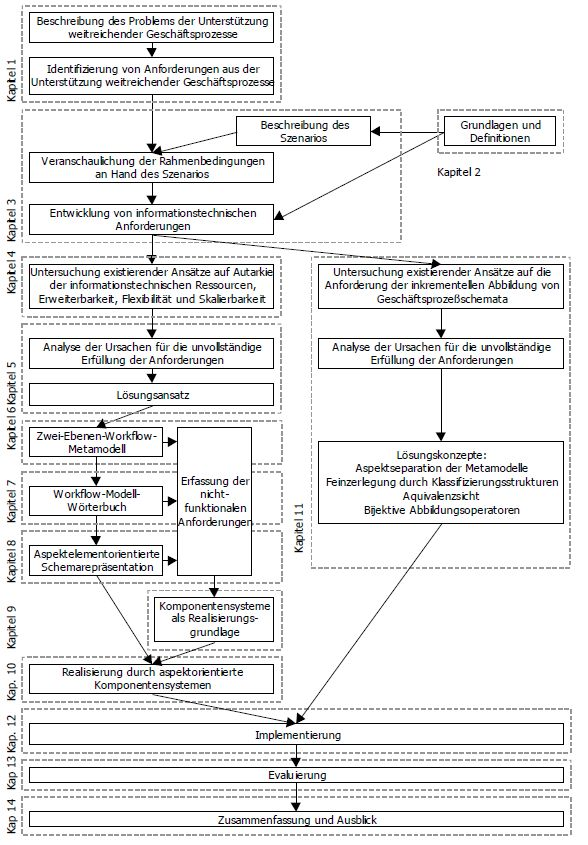
\includegraphics[height=0.9\textheight]{images/ausarbeitung.jpg}
%  \caption{vorgehen nach \autocite{Schmidt:Geschaeftsprozesse}}
%  \label{fig:1}
%\end{figure}


% ---
\chapter{Grundlagen}
\label{cha:grundlagen}

In diesem Kapitel werden die für das Projekt relevanten theoretischen Grundlagen dargestellt. 
Es werden dabei nur Inhalte aufgenommen, die für das Verständnis der Umsetzung und für die Lösung der gestellten Aufgaben notwendig sind. 
Die dargestellten Technologien und Werkzeuge wurden im Rahmen des Projekts praktisch eingesetzt und sind somit problembezogen.




\section{React}
\label{sec:react}
React ist eine von Facebook entwickelte Open-Source-JavaScript-Bibliothek zur Erstellung von Benutzeroberflächen, insbesondere für Single-Page-Applications\autocite{React:Official}. 
Sie erlaubt die komponentenbasierte Entwicklung und unterstützt effizientes Rendering durch ein virtuelles DOM. 
Im vorliegenden Projekt wurde React verwendet, um die interaktive, browserbasierte Benutzeroberfläche für die Scavenger-Hunt-Anwendung zu erstellen.

\section{FastAPI}
\label{sec:fastapi}
FastAPI ist ein modernes, schnelles Webframework für Python, das auf Standards wie OpenAPI und JSON Schema basiert\autocite{FastAPI:Official}. 
Es unterstützt asynchrone Programmierung und bietet eine automatische Generierung von API-Dokumentationen. 
In diesem Projekt dient FastAPI als Backend-Framework zur Implementierung der REST-API, über die das Frontend Daten wie Hunt-Informationen, Benutzerfortschritt und Mediendateien abruft.

\section{PostgreSQL}
\label{sec:postgresql}
PostgreSQL ist ein leistungsstarkes, objektrelationales Open-Source-Datenbanksystem\autocite{PostgreSQL:Official}. 
Es wurde in diesem Projekt für die persistente Speicherung aller Spieldaten genutzt, darunter Benutzerkonten, Hunts, Clues sowie Fortschrittsinformationen.

\section{Traefik}
\label{sec:traefik}
Traefik ist ein moderner Reverse Proxy und Load Balancer für Microservices\autocite{Traefik:Official}. 
In unserem Setup leitet er Aufrufe auf \texttt{werwoelfe.fun} an das Frontend und Anfragen mit \texttt{/api} an das Backend weiter. 
Eine \emph{StripPrefix}-Middleware entfernt dabei das Präfix \texttt{/api}, sodass FastAPI intern ohne \texttt{root\_path} arbeiten kann.



\section{Docker und docker-compose}
\label{sec:docker}
Docker ist eine Plattform zur Containerisierung von Anwendungen, die es erlaubt, Software in isolierten Umgebungen (Containern) auszuführen\autocite{Docker:Official}. 
Mit \texttt{docker-compose} können mehrere Container als zusammenhängender Service-Stack definiert und gestartet werden. 
Im Projekt wurde Docker genutzt, um eine reproduzierbare Entwicklungs- und Produktionsumgebung für Frontend, Backend, Datenbank zu erstellen.

\section{Git und GitHub}
\label{sec:git}
Git ist ein verteiltes Versionskontrollsystem zur Nachverfolgung von Quellcode-Änderungen\autocite{Git:Official}. 
GitHub ist eine webbasierte Hosting-Plattform für Git-Repositories.
Für das Projekt wurden Git und GitHub genutzt, um den Code zu versionieren und die Zusammenarbeit im Team zu koordinieren.
Zusätzlich haben wir das GitHub-Project-Backlog verwendet, um Aufgaben zu planen, den Fortschritt zu verfolgen und die Mitarbeit im Team effizient zu organisieren.


%---
\chapter{Problemanalyse}
\label{cha:problemanalyse}

In diesem Kapitel wird zunächst das übernommene Projekt beschrieben und analysiert, um bestehende Schwachstellen und Herausforderungen zu identifizieren. Anschließend werden die neuen Anforderungen und Zielsetzungen dargestellt, die sich aus den technischen Gegebenheiten sowie den gewünschten funktionalen Erweiterungen ergeben.

\section{Bestandsaufnahme}
Das ursprünglich übernommene Projekt setzte auf eine komplexe Microservice-Architektur mit mehreren eigenständigen APIs, jeweils mit eigener MySQL-Datenbank, RabbitMQ als Message-Bus, Redis als Cache sowie einem Nginx-Proxy. Diese Vielzahl an Containern führte zu einer hohen technischen Komplexität und langen Startzeiten. Für den eigentlichen Anwendungsfall war die Architektur deutlich überdimensioniert, was den lokalen Betrieb und die Einarbeitung neuer Entwickler erheblich erschwerte, insbesondere auf macOS, wo das Setup teilweise gar nicht funktionierte. Insgesamt war das System schwer wartbar, fehleranfällig und bot eine unnötig große Fläche.

\section{Anforderungen/Featureideen}

Die Anforderungen wurden zu Beginn des Projekts gemeinsam mit dem Betreuer abgestimmt und festgelegt. Sie umfassen:

\begin{table}[htbp]
\centering
\begin{tabular}{|p{7cm}|p{7cm}|}
\hline
\textbf{Must have} & \textbf{Should have} \\ \hline
\begin{itemize}
    \item Auf Server aufsetzbar machen und testen (via Docker-Compose oder ähnliches)
    \item Bild und Audio sinnvoll abspeichern 
    \item Accountmanagement und -login
\end{itemize}
& 

\begin{itemize}
    \item UI/UX - individuelle Gestaltung des Startscreens / des Logos / vielleicht auch der Farben der Buttons wäre cool
    \item Info-Button mit den Informationen zur Anwendung (Hochschul-Logo, alle Namen der Entwickler jeweils mit Semester, in dem es bearbeitet wurde, Betreuername
    \item User-Tests wenn es auf Smartphone läuft (wäre auch ohne Accountmanagement denkbar)
\end{itemize}
\\ \hline

\textbf{Could have} & \textbf{Nice to have} \\ \hline

Verwalten der Hunt's 
\begin{itemize}

    \item Auf User-Account speichern zu welchem man Zugang hat
    \item Joinen via QR-Code, Link und HuntID (6 oder 8-Stellige Zahl) ermöglichen
    \item Öffentliche / Private Hunts mit einer Möglichkeit, öffentliche Hunts anzeigen zu lassen (vielleicht auch auf der Karte den Startpunkt anzeigen?)
\end{itemize}

GPS
 \begin{itemize}
     \item Beim Erstellen
     \item Beim spielen überarbeiten
     \item Unterscheidung Zweier Optionen bei GPS: möglichst exakt oder Radius als Trigger (wobei das eigentlich aufs Gleicher rausläuft. Bei Exakt ist die Toleranz halt kleiner - kann man also auch weglassen)
 \end{itemize}
& 
\begin{itemize}
    \item Variante 1: Bei Trigger wird ein AR-Element dargestellt (eigentlich nicht wirklich AR, sondern 3D-Objekt - es sei denn, man versucht, den Boden zu erkennen und platziert das Objekt entsprechend in die Realität)
    \item Variante 2 mit QR-Code als Trigger: direkt über dem QR-Code wird ein AR-Objekt dargestellt. (wahrscheinlich leichter und eher AR)
\end{itemize}

\\ \hline
\end{tabular}
\caption{Anforderungen/Featureideen}
\label{tab:anforderungen}
\end{table}


%---
\chapter{Lösungskonzept}
\label{cha:loesungskonzept}

\section{Architektur- und Technologieentscheidung}
Für das ursprüngliche Projekt wurde .NET Core in einer komplexen Microservice-Struktur eingesetzt. Zwar ist .NET eine leistungsfähige und etablierte Plattform, jedoch brachte sie in diesem Fall mehrere Nachteile mit sich. Die Entwicklungsgeschwindigkeit war geringer, da neue Features oft mehr Konfiguration erforderten. Zudem war die Lernkurve für das Team steiler, da nicht alle Teammitglieder mit C\# und dem .NET-Ökosystem vertraut waren. Insbesondere für Mac- und Linux-Nutzer war die lokale Entwicklungsumgebung umständlicher einzurichten. Für ein Projekt Fokus auf schnelle, iterative Entwicklung war daher ein leichterer, plattformunabhängiger Stack wie React + FastAPI deutlich besser geeignet.

Deswegen wurde im Team besprochen, dass wir die im ursprünglichen Projekt verwendeten Technologien durch React und FastAPI ersetzen wollen. Diese Entscheidung haben wir dem Betreuer vorgestellt, der dem Vorschlag zugestimmt hat.
Die neue Architektur bietet gegenüber der alten .NET-basierten Microservice-Lösung mehrere Vorteile:

\begin{itemize}
    \item Schnelle Entwicklung: FastAPI ermöglicht durch automatische API-Dokumentation, asynchrone Verarbeitung und starke Typisierung eine sehr effiziente Backend-Entwicklung.
    \item Klare Trennung von Frontend und Backend: React und FastAPI arbeiten vollständig entkoppelt, wodurch das Backend auch von anderen Clients (z. B. mobilen Apps) genutzt werden kann.
    \item Leichtgewichtig und flexibel: Im Vergleich zur komplexen Microservice-Architektur ist die neue Lösung einfacher, schneller zu deployen und leichter zu warten.
    \item Starke Python-Integration mit kurzer Lernphase: Python ist leicht verständlich und erlaubt eine schnelle Einarbeitung, was besonders für das Projektteam von Vorteil war.
    \item Moderne Benutzeroberfläche: React ist eine der führenden Frontend-Bibliotheken und bietet eine schnelle, responsive und interaktive UI-Entwicklung.
\end{itemize}

Diese Architektur ist optimal auf die Projektziele abgestimmt, reduziert technische Komplexität und erleichtert sowohl Wartung als auch zukünftige Erweiterungen.

\section{Entwurf der Benutzeroberfläche (Wireframes)}

\begin{figure}[H]
    \centering
    
\includegraphics[width=1\linewidth]{Docs/images/Wireframe.png}
    \caption{Benutzeroberfläche (Wireframe)}
\end{figure}

Nachdem die Entscheidung für die neue Architektur getroffen war, haben wir mit der Erstellung von Wireframes begonnen. Diese dienten als visuelle Entwürfe für die Benutzeroberfläche und halfen, die geplanten Funktionen und Abläufe klar zu strukturieren, bevor die eigentliche Implementierung startete. Im Wireframe wurden die zentralen Benutzerflüsse abgebildet, wie das Erstellen und Beitreten von Hunts, das Anzeigen und Bearbeiten von Fragen, die Verwaltung von Hinweisen sowie grundlegende Profilfunktionen. Durch diese Vorarbeit konnten spätere Missverständnisse vermieden und die Entwicklung effizienter gestaltet werden.

\section{Datenbank Design}
\label{DatenbankDesign}

\begin{figure}[H]
    \centering
    
\includegraphics[width=1\linewidth]{Docs/images/Datenbankschema.png}
    \caption{Datenbankschema}
\end{figure}

Das Datenbankschema wurde mit dbdiagram.io modelliert und bildet die Kernobjekte der Anwendung ab: Benutzer (users), Jagden (hunt), Rätsel/Fragen (clue) sowie den individuellen Spielfortschritt (user\_hunt\_progress, user\_clue\_progress). Primärschlüssel sind ganzzahlige IDs; Relationen sind über Fremdschlüssel definiert.

\subsection{Users}

Die Tabelle users verwaltet die Kontodaten aller Spieler und Ersteller von Hunts. Neben der E-Mail-Adresse und dem gehashten Passwort (verwaltet durch fastapi-users) enthält sie Felder für den Anzeigenamen (username), Spracheinstellungen (language), den Dark-Mode-Status.

\subsection{Hunt}

Die Tabelle hunt beschreibt eine einzelne Schnitzeljagd. Sie speichert einen eindeutigen sechsstelligem Join-Code, den Namen und die Beschreibung der Hunt, Informationen zum Spielort und Startpunkt, den Ersteller (created\_by) sowie Statusangaben zu Sichtbarkeit und Aktivität.

\subsection{Clue}

Die Tabelle clue enthält die einzelnen Rätsel bzw. Aufgaben einer Hunt. Neben Titel, Beschreibung, Hinweisen und der richtigen Antwort können hier auch Medien (Video, Bilder, Audio) sowie verschiedene Fragetypen und Antwortformate hinterlegt werden. GPS-Daten für Fragen und Hinweise werden als JSON-Felder gespeichert, ebenso wie Multiple-Choice-Optionen.

\subsection{User\_hunt\_progress}
Die Tabelle user\_hunt\_progress hält fest, welche Nutzer an welcher Hunt teilnehmen, und speichert zusätzlich den individuellen Spielfortschritt. Neben den Fremdschlüsseln zu user\_id und hunt\_id verweist sie auf den aktuell bearbeiteten Hinweis (current\_clue\_id).

\subsection{User\_clue\_progress}
Die Tabelle user\_clue\_progress erfasst, welche Hinweise ein Spieler bereits gelöst hat, und speichert dazu den Status.

\vspace{2em}
Das Schema ist so aufgebaut, dass es sowohl den Spielbetrieb als auch die Verwaltung und Auswertung von Hunts effizient unterstützt. JSON-Felder sorgen für Flexibilität bei ortsbasierten Aufgaben oder variablen Antwortmöglichkeiten, während eindeutige Schlüssel und Fremdschlüsselbeziehungen Datenkonsistenz gewährleisten.
%---
\chapter{Implementierung}
\label{cha:implementierung}

In diesem Kapitel wird die praktische Umsetzung des in Kapitel \ref{cha:loesungskonzept} beschriebenen Lösungskonzepts erläutert.  
Der Fokus liegt auf der konkreten technischen Realisierung, den eingesetzten Technologien sowie der Integration der einzelnen Komponenten zu einer funktionsfähigen Anwendung.  
Dazu werden zunächst die Implementierungsdetails des Frontends und Backends vorgestellt, gefolgt von einer Beschreibung der Datenbankanbindung, der API-Schnittstellen sowie der eingesetzten Infrastruktur.  
Besonderes Augenmerk wird auf die Interaktion zwischen Client und Server, die Asynchronität der Datenverarbeitung und die Sicherstellung einer benutzerfreundlichen Bedienung gelegt.  

\section{Frontend}

Das Frontend der Anwendung wurde mit \texttt{React 19} implementiert und bildet die Benutzerschnittstelle zur Interaktion mit der Applikation.  
Durch den Einsatz von \texttt{Vite} als Build-Tool konnte eine schnelle Entwicklungsumgebung mit Hot-Reloading und optimierten Builds realisiert werden.  
Für die Client-seitige Navigation kommt \texttt{React Router} zum Einsatz, wodurch ein nahtloses Umschalten zwischen verschiedenen Ansichten ohne vollständiges Neuladen der Seite möglich ist.  
Interaktive Kartenfunktionen werden über die JavaScript-Bibliothek \texttt{Leaflet} bereitgestellt, während \texttt{React-QR-Code} zur Generierung von QR-Codes verwendet wird.

\subsection{Gestaltung und Aufbau}
Die Gestaltung des Frontends basiert auf einem zuvor erstellten Wireframe, der als Grundlage für die Anordnung der Bedienelemente und die Struktur der Navigation diente.  
Dabei lag der Fokus insbesondere auf der intuitiven Bedienbarkeit, einer klaren Informationshierarchie sowie der Minimierung unnötiger Klickpfade.  
Ziel war es, den Nutzern durch eine übersichtliche und konsistente Gestaltung einen reibungslosen Ablauf zu ermöglichen.

\subsection{Navigation}
Die primäre Navigation erfolgt über eine am unteren Bildschirmrand platzierte Navigationsleiste, die aus drei Radio-Buttons besteht.  
Diese ermöglichen den Wechsel zwischen den Hauptseiten \texttt{/home}, \texttt{/profile} und \texttt{/hunt}.  
Jede dieser Hauptseiten ist funktional klar abgegrenzt und deckt spezifische Anwendungsfälle ab.

\subsubsection{Home-Seite}
Die Startseite bietet zwei zentrale Aktionen: den Beitritt zu einer Hunt oder das Erstellen einer neuen Hunt.  
Ein Beitritt ist auch ohne Benutzerkonto als Gast möglich; eingeloggte Benutzer profitieren jedoch von einer Fortschrittsspeicherung.  
Die Interaktion folgt dabei einem festen Ablauf:  
\begin{enumerate}
    \item Auswahl der Option \enquote{Hunt beitreten}  
    \item Eingabe einer Hunt-ID, Öffnen eines Einladungslinks oder Scannen eines QR-Codes  
    \item Weiterleitung zur \texttt{/StartHunt}-Seite mit einer Übersicht und der Möglichkeit, die Hunt zu starten oder zu verlassen  
    \item Start der Hunt mit Wechsel zur \texttt{/PlayHunt}-Seite
\end{enumerate}

Für das Erstellen einer Hunt ist eine Anmeldung erforderlich.  
Nach Eingabe eines Namens wird der Nutzer auf die \texttt{/EditHunt}-Seite geleitet, um Metadaten zu hinterlegen und Fragen zu erstellen.  
Über den \enquote{Edit Question}-Button kann auf die \texttt{/EditQuestion}-Seite gewechselt werden, um Inhalte, Lösung und optionale Hinweise zu definieren.

\subsubsection{Profile-Seite}
Auf dieser Seite können sich Nutzer registrieren, einloggen sowie Sprache und Erscheinungsbild (Hell-/Dunkelmodus) anpassen.  
Zu dieser Seite wird man ebenfalls weitergeleitet, wenn ein nicht eingeloggter Nutzer versucht, auf eine loginpflichtige Funktion zuzugreifen.

\subsubsection{Hunts-Seite}
Diese Ansicht listet alle Hunts auf, die einem Nutzer zugeordnet sind: beigetretene, selbst erstellte und öffentlich zugängliche Hunts.  
Über drei Radio-Buttons am oberen Bildschirmrand lässt sich zwischen den Kategorien \enquote{Beigetreten}, \enquote{Eigene} und \enquote{Durchsuchen} umschalten.  
Ein Klick auf eine Hunt in den Bereichen \enquote{Beigetreten} oder \enquote{Durchsuchen} führt zur zugehörigen \texttt{/StartHunt}-Seite, während eigene Hunts zur \texttt{/EditHunt}-Seite verlinken.

\section{Backend}

Das Backend der Anwendung wurde mit FastAPI implementiert und bildet die zentrale Schnittstelle zwischen Frontend, Datenbank.
Es stellt sämtliche API-Endpunkte bereit, verarbeitet Anfragen asynchron und verwaltet Authentifizierung, Spiellogik sowie den Zugriff auf gespeicherte Daten.
Durch den Einsatz von FastAPI konnten wir eine klare Trennung zwischen Geschäftslogik, Datenbankzugriff und Routen-Definition erreichen.
In den folgenden Kapiteln wird schrittweise erläutert, wie die einzelnen Komponenten des Backends aufgebaut sind und zusammenarbeiten.

\subsection{Datenbank-Implementierung}
PostgreSQL wird als relationale Datenbank verwendet.
Die Anbindung erfolgt über SQLAlchemy in Kombination mit AsyncSession, sodass alle Datenbankoperationen asynchron ausgeführt werden können.
Das sorgt für bessere Skalierbarkeit und verhindert, dass langlaufende Abfragen den Eventloop blockieren.

Die Tabellenstruktur entspricht dem in Kapitel 4.3 beschriebenen Datenbankschema.
Jede Tabelle ist als Python-Klasse definiert, die von der gemeinsamen Basisklasse \texttt{Base} erbt.
Die Spalten werden mithilfe von SQLAlchemy-Spaltentypen (\texttt{Column}, \texttt{String}, \texttt{Integer}, \texttt{Boolean}, \texttt{JSON}, \texttt{DateTime} etc.) definiert,
wobei Primär- und Fremdschlüssel zur Wahrung der Datenintegrität genutzt werden.

Ein Beispiel ist die Tabelle \texttt{Hunt}, die Informationen zu einer Schnitzeljagd speichert.
Dabei wird ein eindeutiger sechsstelliger Code automatisch generiert, der es ermöglicht, einer Hunt ohne Kenntnis der internen Datenbank-ID beizutreten.

Die Verbindung zur Datenbank wird zentral in einer Konfigurationsdatei hergestellt,
wobei der Verbindungsstring \texttt{DATABASE\_URL} aus den Umgebungsvariablen (\texttt{.env}) gelesen wird.
So kann dieselbe Codebasis sowohl lokal als auch in der Produktionsumgebung genutzt werden, ohne die Zugangsdaten im Quellcode zu hinterlegen.

Die Verbindung zur PostgreSQL-Datenbank wird im Projekt über einen Connection String definiert:
\begin{verbatim}
DATABASE_URL=postgresql+asyncpg://postgres:1967@db:5432/scavengerhunt
\end{verbatim}

Dieser String gibt alle nötigen Informationen für den Verbindungsaufbau an:  
\texttt{postgresql+asyncpg} legt den Datenbanktyp (PostgreSQL) und den verwendeten asynchronen Treiber (\texttt{asyncpg}) fest.  
\texttt{postgres} ist der Benutzername, \texttt{1967} das Passwort, \texttt{db} der Hostname des Datenbankcontainers im Docker-Netzwerk, \texttt{5432} der Standard-Port von PostgreSQL und \texttt{scavengerhunt} der Name der zu verwendenden Datenbank.  


\subsection{Asynchrones Backend}

Das Backend der Anwendung ist vollständig asynchron aufgebaut.  
Dies bedeutet, dass Anfragen nicht blockierend verarbeitet werden, sondern die Ausführung während externer Operationen (z.~B. Datenbankzugriffe, API-Calls) pausiert werden kann, um in dieser Zeit andere Anfragen zu bearbeiten.  

Technisch basiert dies auf den asynchronen Funktionen von \texttt{FastAPI}.
Die Funktionen sind mit dem Schlüsselwort \texttt{async} definiert und verwenden \texttt{await}, um auf Ergebnisse von Operationen zu warten, ohne den Haupt-Thread zu blockieren.  

Für den Datenbankzugriff wird der asynchrone SQLAlchemy-Engine-Typ verwendet, zusammen mit dem Treiber \texttt{asyncpg}.  
Dadurch können auch komplexe Datenbankabfragen effizient ausgeführt werden, selbst wenn viele Nutzer gleichzeitig auf das System zugreifen.

Der Einsatz eines asynchronen Backends bietet insbesondere folgende Vorteile:
\begin{itemize}
    \item Höhere Skalierbarkeit bei gleichzeitigen Anfragen
    \item Bessere Reaktionszeiten unter Last
    \item Ressourcenschonendere Verarbeitung im Vergleich zu synchronen Blockierungen
\end{itemize}

\subsection{Benutzerverwaltung mit JWT und FastAPI Users}

Die Benutzerverwaltung der Anwendung basiert auf dem Paket \texttt{fastapi-users}.  
Dieses bietet eine vollständige Implementierung für Benutzer-Authentifizierung, -Registrierung und -Verwaltung und unterstützt dabei verschiedene Authentifizierungsstrategien wie E-Mail/Passwort oder OAuth\autocite{fastapi-users:Official}.
Für dieses Projekt wurde die Authentifizierung per JWT (JSON Web Token) gewählt.

JWT ist ein kompaktes und sicheres Format zur Übertragung von Anfragen zwischen zwei Parteien. Nach erfolgreicher Anmeldung erhält der Client ein signiertes Token, das bei jeder weiteren Anfrage im \texttt{Authorization-Header} mitgesendet wird.  
Das Backend überprüft die Signatur und extrahiert die Benutzerinformationen, ohne eine zusätzliche Datenbankabfrage durchführen zu müssen.

Die Integration von \texttt{fastapi-users} erfolgt über einen \texttt{UserManager}, 
der die Logik für Benutzeroperationen enthält und das Passwort-Hashing, 
das Erstellen von Tokens übernimmt.  
Die Funktion \texttt{get\_user\_db} stellt der Bibliothek den Datenbankzugriff 
per \texttt{SQLAlchemyUserDatabase} bereit.  

Für die Authentifizierung wird ein \texttt{AuthenticationBackend} mit 
\texttt{JWTStrategy} konfiguriert. Dabei werden ein geheimer Schlüssel 
(\texttt{SECRET\_KEY}) und die Gültigkeitsdauer der Tokens definiert.  
Über den \texttt{BearerTransport} wird festgelegt, dass Tokens im 
\texttt{Authorization}-Header gesendet werden.  

Die so konfigurierten Router (\texttt{get\_auth\_router}, \texttt{get\_register\_router} ...) werden anschließend in die Hauptanwendung eingebunden.  
Dies ermöglicht eine vollständige Benutzerverwaltung mit minimalem Implementierungsaufwand, 
da Authentifizierung, Autorisierung und Benutzeraktionen direkt über die 
bereitgestellten Endpunkte erfolgen.

\subsection{API-Endpunkte}

Die Schnittstellen des Backends sind nach den Prinzipien von REST aufgebaut und über eindeutige URLs erreichbar. 
Jede Route ist dabei einer HTTP-Methode zugeordnet, um die gewünschte Aktion eindeutig zu definieren. 
Die Implementierung erfolgt asynchron mit FastAPI, wodurch Anfragen parallel verarbeitet werden können. 
Die Authentifizierung erfolgt, falls erforderlich, über JWT-Token und den Mechanismus von \texttt{fastapi-users}. 
Für alle sensiblen Operationen ist der eingeloggte Benutzer (\texttt{current\_user}) als Abhängigkeit hinterlegt.

\subsubsection{GET-Endpunkte}
\begin{itemize}
    \item Abrufen einzelner Entitäten wie einer spezifischen Hunt oder eines Clues.
    \item Listen von Ressourcen (z. B. alle Hunts eines Benutzers, alle öffentlichen Hunts, alle Clues zu einer Hunt).
    \item Abruf von Informationen wie dem aktuellen Fortschritt eines Spielers.
    \item Bereitstellung statischer Dateien wie hochgeladener Bilder oder Audiodateien.
\end{itemize}

\subsubsection{POST-Endpunkte}
\begin{itemize}
    \item Erstellen neuer Ressourcen, z. B. \texttt{/create-hunt} oder \texttt{/hunts/\{hunt\_id\}/clues}.
    \item Hochladen von Mediendateien (Bilder, Audio) für Clues oder Hinweise.
    \item Teilnahme an einer Hunt über einen sechsstelligen Code.
    \item Speichern von Spielfortschritt, sobald ein Spieler einen Hinweis gelöst hat.
\end{itemize}

\subsubsection{PUT/PATCH-Endpunkte}
\begin{itemize}
    \item Vollständige (\texttt{PUT}) oder teilweise (\texttt{PATCH}) Aktualisierung bestehender Ressourcen.
    \item Beispiele: Änderung von Hunt-Details oder Anpassung eines Clues (Beschreibung, Medien, Antwortoptionen).
\end{itemize}

\subsubsection{DELETE-Endpunkte}
\begin{itemize}
    \item Löschen von Ressourcen wie Hunts oder Clues.
    \item Entfernen eines Spielers aus einer Hunt.
\end{itemize}

Alle Endpunkte sind klar nach Ressourcentypen (\texttt{/hunts}, \texttt{/clues}, \texttt{/images}, \texttt{/audio}) 
strukturiert und nutzen sprechende URLs, um die Funktion sofort erkennbar zu machen. 
Parameter wie \texttt{\{hunt\_id\}} oder \texttt{\{clue\_id\}} identifizieren konkrete Datensätze. 
Das Backend gibt JSON-Antworten zurück, um die direkte Verarbeitung im Frontend zu ermöglichen.

\subsection{Sicherheit und Validierung}

Die Anwendung nutzt durchgängig \texttt{Pydantic}-Modelle zur Validierung von Eingaben.  
Diese Modelle definieren klar den erwarteten Datentyp und erlauben Standardwerte sowie optionale Felder.  
Ungültige Eingaben werden bereits vor der Ausführung abgefangen, wodurch fehlerhafte oder schadhafte Daten nicht in die Datenbank gelangen können.

\paragraph{Input-Validierung}
Für API-Endpunkte wie das Erstellen oder Aktualisieren von Hunts und Clues werden spezielle Pydantic-Schemas verwendet.  
Diese prüfen, ob alle Pflichtfelder vorhanden sind, ob Datentypen korrekt sind (z.\,B. \texttt{int} für IDs, \texttt{bool} für Statusfelder) und ob optionale Felder korrekt formatiert sind.

\paragraph{Datei-Uploads}
Datei-Uploads (Bilder und Audiodateien) werden über FastAPIs \texttt{UploadFile} behandelt.  
Es erfolgt eine Prüfung der Dateiendung und des MIME-Typs, um nur erlaubte Formate zu akzeptieren.  
Zudem können maximale Dateigrößen über Server-Konfiguration begrenzt werden, um Missbrauch zu verhindern.

\paragraph{Sicherheit}
Die Kombination aus \texttt{Pydantic}-Validierung und Upload-Prüfungen reduziert das Risiko von Sicherheitslücken wie SQL-Injection oder fehlerhafter Verarbeitung schadhafter Dateien.  
Darüber hinaus sorgen Authentifizierung über JWT sowie Berechtigungsprüfungen (\texttt{current\_user}) dafür, dass nur autorisierte Nutzer auf geschützte Ressourcen zugreifen können.



%---
\chapter{Inbetriebnahme}
\label{cha:inbetriebnahme}

Dieses Kapitel beschreibt die Schritte, die notwendig sind, um die entwickelte WebApp sowohl lokal als auch auf einem Server in Betrieb zu nehmen.  
Da sich die Anforderungen an eine lokale Entwicklungsumgebung und ein produktives Deployment deutlich unterscheiden, wurden zwei separate \texttt{docker-compose}-Dateien erstellt:  
eine für schnelle, unkomplizierte Tests auf dem Entwicklerrechner und eine für den Betrieb der Anwendung auf dem Zielserver inklusive SSL-Unterstützung.

\subsection{Lokale Inbetriebnahme}

Die \texttt{docker-compose}-Datei für lokale Tests enthält keine besonderen Anpassungen und kann direkt mit dem Befehl

\begin{verbatim}
docker compose -f docker-compose-local.yaml up --build
\end{verbatim}

ausgeführt werden.  
Anschließend ist die Anwendung unter \texttt{http://localhost:3000} erreichbar.

\subsection{Deployment auf dem Server}

Das Ausrollen der WebApp auf dem Server stellte sich an einigen Stellen als herausfordernd heraus.  
Als Server kam ein UGreen NAS zum Einsatz. Zunächst mussten wir uns mit dem NAS vertraut machen und prüfen, wie wir unseren Source-Code darauf übertragen, einfach aktualisieren und Docker effektiv nutzen können.  

Wir kamen zu dem Ergebnis, dass es am einfachsten ist, sich per \texttt{ssh} mit dem NAS zu verbinden und anschließend mit

\begin{verbatim}
git pull
docker compose up --build
\end{verbatim}

das Projekt zu aktualisieren und neu zu deployen.  
Die grafische Benutzeroberfläche des NAS erwies sich ebenfalls als hilfreich, da sich in der Docker-App schnell erkennen ließ, ob Probleme mit einem Container vorlagen und die Logs einfach eingesehen werden konnten.  

Zusätzlich wurde am Router der Port \texttt{3000} freigegeben, um einen Zugriff von außen zu ermöglichen.

Dies funktionierte problemlos, bis wir ein SSL-Zertifikat einbinden wollten, um die Seite über \texttt{https} (statt \texttt{http}) erreichbar zu machen. Hierfür setzten wir \texttt{Traefik} ein – einen Reverse Proxy mit automatischer SSL-Zertifikatsverwaltung.  

Die Einbindung von Traefik erforderte jedoch einige Änderungen an der \texttt{docker-compose}-Datei, was das lokale Testen unnötig erschwerte.  
Aus diesem Grund entschieden wir uns, eine zweite \texttt{docker-compose}-Datei anzulegen. Über den Parameter

\begin{verbatim}
-f dateiname.yaml
\end{verbatim}

konnte anschließend einfach ausgewählt werden, welche Konfiguration für den Build verwendet werden sollte.

Zudem mussten wir die Routerkonfiguration noch einmal genauer prüfen, da anfangs beim Aufruf von \texttt{https://domain.name} automatisch auf Port~9999 umgeleitet wurde.  
Dies verhinderte, dass Traefik ein SSL-Zertifikat generieren konnte.  
Die Ursache lag in einer automatischen Weiterleitungsfunktion des NAS.  
Nach deren Deaktivierung und der Freigabe des Ports~443 für HTTPS am Router funktionierte die Verbindung.

Allerdings kam es anschließend zu Kommunikationsproblemen mit dem Backend, da sich sowohl die Domain (API-Basis) als auch die Ports geändert hatten.  
Um diese Abhängigkeiten leichter verwalten zu können, haben wir eine Environment-Variable eingeführt, über die sich die Domain zentral anpassen lässt, sodass man sie nur an einer Stelle je für Frontend und Backend ändern muss.  
Nach diesen Anpassungen lief das System stabil und ließ sich einfach warten und aktualisieren.

%---
\chapter{User Tests}

Um die Benutzerfreundlichkeit und Funktionalität der WebApp aus Sicht realer Anwender zu überprüfen, wurden externe User-Tests durchgeführt.  
Hierfür baten wir Bekannte, die Anwendung zu nutzen und typische Anwendungsfälle auszuführen.  

Zur strukturierten Erfassung der Rückmeldungen setzten wir eine Google-Forms-Umfrage ein.  
Diese enthielt sowohl geschlossene Fragen (z.\,B. zur Bewertung von Bedienbarkeit, Design und Performance auf einer Skala von 1 bis 5) als auch offene Fragen für detailliertes Feedback.  

\section{Ergebnisse der Umfrage}

Die Auswertung der Umfrage zeigte, dass die Anwendung insgesamt als intuitiv und optisch ansprechend wahrgenommen wurde.  
Gleichzeitig erhielten wir wertvolle Hinweise zu kleineren Verbesserungsvorschlägen, beispielsweise bei der Anordnung einzelner Bedienelemente oder der Optimierung von Eingabefeldern auf mobilen Geräten.  

\begin{itemize}
    \item Wie zufrieden sind Sie insgesamt mit der Web-App? Durchschnitt: 4
    \item Wie einfach war es, mit einem Code an einer bestehenden Schnitzeljagd teilzunehmen? Durchschnitt: 5
    \item Wie einfach war es, eine neue Schnitzeljagd zu erstellen und eine Frage hinzuzufügen? Durchschnitt: 4
    \item Wie intuitiv war das Lösen der ersten Frage in einer öffentlichen Schnitzeljagd? Durchschnitt: 4.25
    \item Wie bewerten Sie die Gesamtbenutzerfreundlichkeit der App? Durchschnitt: 4.25
\end{itemize}

\section{Fazit der User Tests}

Das gesammelte Feedback half uns, gezielte Optimierungen vorzunehmen und die Benutzererfahrung insgesamt zu verbessern.  
Insbesondere konnten wir durch die Rückmeldungen konkrete Anpassungen an der Navigation und der Anordnung von Bedienelementen vornehmen sowie die Limitierung von Eingaben in Eingabefeldern.  
Diese iterative Anpassung hat dazu beigetragen, die Anwendung stabiler, ansprechender und einfacher zu bedienen zu machen.

%---
\chapter{Evaluierung}
\label{cha:evaluierung}

In diesem Kapitel wird bewertet, inwieweit die zu Beginn der Arbeit definierten Ziele erreicht wurden.  
Dabei erfolgt ein Abgleich der geplanten Anforderungen mit den tatsächlich umgesetzten Funktionen und Ergebnissen.  

\section{Erreichte Ziele}

\subsection{Must-Have Anforderungen}

Die essenziellen Kernfunktionen, die als „Must-Have“ definiert wurden, konnten vollständig implementiert und erfolgreich getestet werden:  

\begin{itemize}
  \item \textbf{Server-Deployment:} Die WebApp lässt sich mittels \texttt{docker-compose} problemlos auf einem Server aufsetzen und betreiben.  
  Dies umfasst sowohl den initialen Aufbau als auch einfache Aktualisierungen über Git und Docker.  
  \item \textbf{Bild- und Audioverwaltung:} Medieninhalte wie Bilder und Audiodateien werden sinnvoll gespeichert und verarbeitet, sodass sie in der Anwendung abrufbar sind.  
  \item \textbf{Accountmanagement und Login:} Ein funktionsfähiges Nutzerverwaltungssystem inklusive Registrierung, Authentifizierung und Login wurde realisiert.  
  Dies bildet die Grundlage für personalisierte Funktionen und zukünftige Erweiterungen.  
\end{itemize}

\subsection{Should-Have Anforderungen}

Die meisten Funktionen aus der Kategorie „Should-Have“ wurden ebenfalls umgesetzt und tragen zur besseren Benutzererfahrung bei:  

\begin{itemize}
  \item \textbf{Individuelle UI/UX-Gestaltung:} Das Logo sowie auf der Startseite lässt sich über eine Konfigurationsdatei Anpassen, um eine ansprechende Oberfläche zu schaffen.  
  \item \textbf{Info-Button:} Ein Informationsbutton wurde integriert, der wichtige Angaben zur Anwendung enthält, darunter die Namen aller Entwickler sowie der Betreuername. Der Inhalt des Infotextes lässt sich ebenfalls über die Konfigurationsdatei anpassen.
  \item \textbf{User Tests:} Um die Anwendung aus Sicht realer Nutzer zu evaluieren, wurden Tests mit Bekannten durchgeführt, insbesondere auch auf Smartphones. Die Rückmeldungen wurden systematisch über Google Forms gesammelt und lieferten wertvolle Hinweise zur Optimierung.  
\end{itemize}

\subsection{Could-Have Anforderungen}

Alle als „Could-Have“ definierten Funktionen konnten erfolgreich umgesetzt werden:  

\begin{itemize}
  \item \textbf{Verwaltung der Hunts:} Hunts können nun über User-Accounts verwaltet werden, inklusive Zugriffssteuerung.  
  \item \textbf{Beitritt zu Hunts:} Nutzer können Hunts per QR-Code, Link oder HuntID (6- oder 8-stellige Zahl) beitreten. 
  \item \textbf{Öffentliche und private Hunts:} Es besteht die Möglichkeit, öffentliche Hunts anzuzeigen über den "Browse" Reiter oder seine Hunts privat zu stellen. Ebenso kann man eine Hunt als inaktiv zu markieren, wenn sie Beispielsweise aufgrund fehlender Hinweise, welche am Ort versteck werden müssen, nicht spielbar ist.
  \item \textbf{GPS-Funktionalitäten:} GPS-Daten werden sowohl beim Erstellen als auch beim Spielen erfasst und verarbeitet. Der GPS-Standpunkt kann wahlweise als exakte Position oder als Radius definiert werden. 
\end{itemize}

\section{Nicht realisierte Ziele}

Die „Nice-To-Have“-Funktionen, insbesondere die Augmented-Reality-Elemente, konnten aufgrund des Zeitrahmens nicht umgesetzt werden:  

\begin{itemize}
  \item \textbf{AR-Elemente bei Triggern:} Die Darstellung von 3D-Objekten als AR-Elemente bei Positions- oder QR-Code-Triggern wurde nicht realisiert.  
  Dies stellt jedoch eine vielversprechende Option für zukünftige Erweiterungen dar.  
\end{itemize}

\section{Bewertung und Ausblick}

Insgesamt konnten alle wesentlichen Projektziele vollständig erreicht werden.  
Das Projekt bietet eine stabile und funktionale Grundlage für den produktiven Einsatz der WebApp.  

Die erfolgreiche Umsetzung der Kern- und Zusatzfunktionen, einschließlich der umfangreichen GPS- und Hunt-Verwaltung, zeigt den hohen Reifegrad der Anwendung.  

Die durchgeführten User Tests bestätigen die gute Usability und liefern wertvolles Feedback für zukünftige Verbesserungen. 

Die noch offenen „Nice-To-Have“-Features sind interessante Erweiterungsmöglichkeiten, die in Folgeprojekten integriert werden können, um das Nutzererlebnis weiter zu steigern.  

Zusammenfassend lässt sich festhalten, dass die Arbeit erfolgreich war und eine solide Basis für den weiteren Ausbau der Anwendung geschaffen wurde.

%---
\chapter{Zusammenfassung und Ausblick}
\label{cha:zusammenfassung}

\section{Erreichte Ergebnisse}
\label{sec:ergebnisse}

Im Rahmen dieses Projekts wurde eine WebApp entwickelt, die erfolgreich auf einem Server mittels \texttt{docker-compose} deploybar ist.  
Die Kernfunktionen wie Bild- und Audioverwaltung sowie ein Accountmanagement mit Login wurden vollständig umgesetzt.  
Darüber hinaus wurden zahlreiche Zusatzfunktionen realisiert, darunter eine individualisierte Benutzeroberfläche mit Startbildschirm, Logo und ein Info-Button mit relevanten Projektinformationen.  
Die durchgeführten User-Tests bestätigten die gute Benutzerfreundlichkeit und lieferten wertvolles Feedback zur Optimierung.  
Besonders hervorzuheben ist die vollständige Integration der Verwaltung und Teilnahme an Hunts inklusive GPS-Funktionalitäten.  
Somit konnten alle wesentlichen Ziele erreicht und der Fortschritt nachgewiesen werden.  

\section{Ausblick}
\label{sec:ausblick}

Das Projekt bietet eine solide Grundlage, die in verschiedenen Richtungen weiterentwickelt werden kann.  
Im Folgenden werden Ideen zur Erweiterung und Übertragbarkeit der Lösung vorgestellt, um den Nutzen der Arbeit zu erhöhen und neue Anwendungsfelder zu erschließen.  

\subsection{Erweiterbarkeit der Ergebnisse}
\label{sub:erweiterbarkeit}

Die modulare Architektur der WebApp bietet vielfältige Möglichkeiten zur Erweiterung und Verbesserung der bestehenden Funktionen.  
Eine vielversprechende Erweiterung wäre die Integration von Augmented-Reality-Elementen, wodurch 3D-Objekte direkt in die reale Umgebung eingebettet werden könnten, um die Nutzererfahrung interaktiver und immersiver zu gestalten.  

Darüber hinaus könnte ein sogenanntes Hunt Creator Dashboard implementiert werden, das Erstellern von Hunts erlaubt, den Spielverlauf in Echtzeit zu verfolgen.  
Dies würde eine bessere Kontrolle und Analyse des Nutzerverhaltens ermöglichen sowie eine Möglichkeit für den Creator zu schauen, wer wie weit ist, um eventuell einen Preis für den schnellsten Spieler zu vergeben. 

Eine weitere sinnvolle Erweiterung ist die Einführung von Filtermöglichkeiten beim Durchsuchen der verfügbaren Hunts.  
Beispielsweise könnten Nutzer Hunts gezielt nach GPS-Regionen oder anderen Kriterien filtern, um schneller passende Spiele zu finden.  

Für GPS-basierte Fragen könnte die Anwendung den aktuellen Standort des Spielers live auf der Karte anzeigen, wodurch Orientierung und Interaktion erleichtert würden.  

Im Bereich der Nutzerverwaltung wäre es hilfreich, wenn bei Ablauf oder Verlust des Login-Tokens automatisch eine Login-Maske eingeblendet wird, um eine unterbrechungsfreie Nutzung der App zu gewährleisten.  

Nicht zuletzt kann durch die Implementierung von Ladeanzeigen an wichtigen Stellen, wie etwa während der Standortaktualisierung oder beim Laden von Bildern und Videos aus der Datenbank, die Benutzerfreundlichkeit deutlich gesteigert werden, da Nutzer stets über laufende Prozesse informiert sind.  

\subsection{Übertragbarkeit der Ergebnisse}
\label{sub:uebertragbarkeit}

Die entwickelten Konzepte und Technologien sind nicht auf den konkreten Anwendungsfall beschränkt, sondern können auch auf andere Problemstellungen übertragen werden.  
So lässt sich das Accountmanagement, die Medienverwaltung und die GPS-basierte Interaktion beispielsweise in anderen Location-based Services, Lern-Apps oder Event-Management-Systemen einsetzen.  
Die Nutzung von Traefik als Reverse Proxy mit automatischer SSL-Zertifikatsverwaltung ist eine Best-Practice-Lösung, die in vielen Webprojekten Anwendung finden kann.  
Darüber hinaus bieten die User-Test-Methodik und die Nutzung von Containerisierung gute Beispiele für die Umsetzung agiler und wartbarer Softwareprojekte.  
Somit liefert diese Arbeit wertvolle Erkenntnisse und eine Basis, die über das ursprüngliche Projekt hinaus von Nutzen sein kann.

%-----------------------------------------------------------------------
\appendix

%---
\printbibliography[heading=bibintoc]

%---

\end{document}